\chapter{Konfiguration des Betriebssystems}

Ein essentieller Punkt zu Beginn des Projektes ist die Auswahl des Betriebssystems, da im weiteren Verlauf alle Entwicklungen darauf aufbauen werden. Außerdem ist ein Teilziel des Projektes, schon existierende Software zu nutzen, um den Entwicklungsaufwand klein zu halten und den Fokus auf die eigentliche Fragestellung zu richten. Also habe ich das bereits auf dem BeagleBone vorinstallierte Betriebssystem - {\AA}ngström Linux - intensiv getestet.\\

\noindent Die grundlegenden Fragen waren:

\begin{itemize}
  \item Gibt es genügend Speicherplatz für die zu entwickelnde Software?\\
  Wie schaffe ich bei Bedarf weiteren Speicherplatz für meine Anwendungen?
  \item Wird die zusätzlich gebrauchte Software (Webserver, FTP-Server, etc...) in einem Repository zur Verfügung gestellt?
  \item Sind ausreichend Rechenleistung und Arbeitsspeicher verfügbar, um zusätzliche Dienste zu betreiben?
  \item Sind die benötigten Systemressourcen (Netzwerkports u.a.) verfügbar, bzw. kann ich sie ohne großen Aufwand freigeben?
\end{itemize}

Die Tests ergaben, dass das Betriebssystem mit einer graphischen Oberfläche und mehreren Netzwerkdiensten ausgeliefert wird. 
Die graphische Oberfläche verbraucht Systemressourcen und Speicherplatz, ist aber überflüssig, da das System headless betrieben werden soll. Dazu laufen ein Apache Webserver, eine Cloud9 Entwicklungsumgebung und ein Websocket Server. Des weiteren verwendet {\AA}ngström Distribution parallel zwei verschiedene Daemon Manager (\gls{systemd} und \gls{sysvinit}). Diese erschweren das Arbeiten mit {\AA}ngström Linux erheblich.

Die Software, die ich für mein Projekt verwenden möchte, liegt nicht in den offiziellen Repositories vor. Also müßte ich sie selber konfigurieren und kompilieren.

Aus diesen Erfahrungen folgt, dass {\AA}ngström Linux nicht das richtige Betriebssystem für mein Projekt ist. Der Aufwand, es an meine Bedürfnisse anzupassen, wäre größer als auf eine andere Distribution zurückzugreifen.\\

Die zweite vom Hersteller des BeagleBone angebotene Distribution ist Debian Linux. Auch diese habe ich nach den oben genannten Kriterien geprüft. Die Konfiguration, die schon zum Ausschluss von {\AA}ngströn Linux führte, fanden sich im Prinzip auch hier. Auf \href{http://www.armhf.com/}{ARMhf.com} gibt es zwar eine weitere Debian-Installation bereits fertig als Linux Image. Diese hat nicht die oben erwähnten Eigenheiten, nutzt aber die neueste Kernel-Version, die mit der Bonescript Library nicht kompatibel ist. Ein Kernel-Downgrade wäre möglich, ist aber grundsätzlich und unter Debian im Besonderen sehr aufwändig. Daher eignet sich Debian Linux ebenfalls nicht für mein Projekt.\\

Eine weitere Distribution für BeagleBone ist Arch Linux. Die Besonderheit dieser Distribution ist, dass die Basisinstallation sehr Ressourcen schonend ist. Sie enthält keinerlei Software, die nicht für den grundsätzlichen Betrieb erforderlich ist. Gleichzeitig stellt sie Werkzeuge zur Verfügung, um die benötigte Software bequem aus umfangreichen Repositories zu installieren. Abweichend von der regulären Kernel-Entwicklung wird die hier benötigte Kernel-Version (3.8) und entsprechende Header Files über die Pakete \textit{linux-am33x-legacy} und \textit{linux-headers-am33x-legacy} bereitgestellt.\\

Somit ist meines Erachtens Arch Linux das richtige Betriebssystem für dieses Projekt. Darüber hinaus kenne ich es seit langem, da ich es beruflich wie privat auf Desktop Computern verwende. Ich muss mich also nicht in eine neue Distribution einarbeiten.


\section{Software}

Zusätzlich zu den mitgelieferten Pakteten der Distribution werden noch einige zusätliche Pakete benötigt, die aber keiner besonderen Konfiguration benötigen und daher hier nicht näher erklärt sind. In der Tabelle \ref{tab:additionalPackages} findet sich eine Liste mit diesen Paketen.\\

Desweiteren werden ein HTTP-Server und die JavaScript Engine für den WebSocket Server benötigt. Der Proxy-Server sorgt dafür, dass die Seite von außen über einen einzigen Port erreichbar ist und dass mit geringem Aufwand \gls{ssl}-verschlüsselte Verbindungen hergestellt werden können. Zusätzlich wird noch ein FTP-Server installiert, um Messdaten ohne Webinterface abrufen zu können (Abb. \ref{fig:componentsServer}).

\begin{figure}[ht]
  \centering
  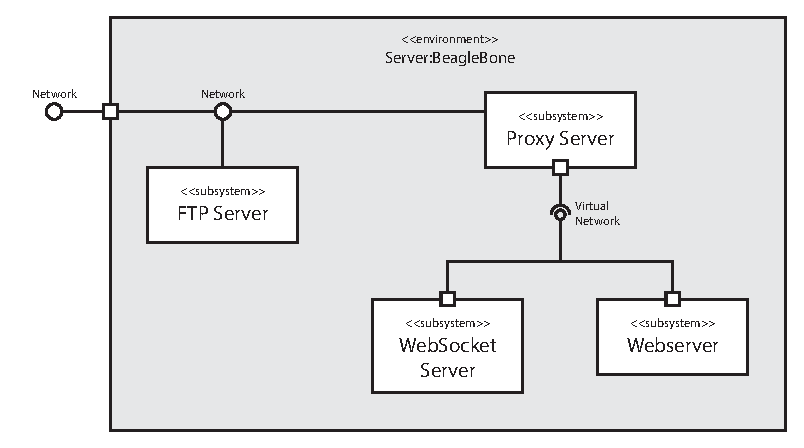
\includegraphics[width = 0.8\textwidth]{dokumentation/images/componentsServer.eps}
  \caption{Komponenten des boneserver}
  \label{fig:componentsServer}
\end{figure}


\subsection{Proxy Server -- HAProxy}
\label{subsec:HAProxy}
HAProxy ist ein Proxy-Server, der eigentlich eingesetzt wird, um Anfragen via \gls{tcp} auf mehrere Server zu verteilen. Wesentlich interessanter für diese Arbeit ist allerdings, dass der HAProxy, ab Version 1.5, sog. \gls{ssl-offloading} unterstützt und nativ \gls{ssl}-verschlüsselte Verbindungen verarbeiten kann. Dabei erfüllt bereits eine einfache Basis-Konfiguration bereits diese Aufgabe \cite{kuehnast2014}.

In diesem Projekt wird HAProxy eingesetzt, um WebSocket Requests von regulären HTTP Requests zu trennen und auf unterschiedliche Dienste weiterzuleiten. Ziel dieser Maßnahme ist es, nach außen die gesamte Website hinter einem Port zu betreiben, obwohl die beiden Prozessen völlig von einander getrennt sind. So ist die Gefahr minimal, dass bei einem Feldeinsatz der Port für den WebSocket Server von einer Firewall blockiert wird. Die Website ist somit entweder vollständig erreichbar oder gar nicht. Auch ist der WebSocket Server, der systembedingt mit root-Rechten laufen muss, ausschließlich per WebSocket über den Proxy-Server zu erreichen und so gegenüber Angriffen von außen weitgehend sicher.

Ein weiterer wichtiger Punkt ist, dass sich für jeden Server die maximale Anzahl der aktiven Verbindungen bequem per Konfigurationsdatei einstellen lassen. So wird ohne besondere Programmierung sichergestellt, dass immer nur eine Verbindung zum WebSocket Server besteht. Alle weiteren Verbindungsanfragen werden auf eine Warteliste gesetzt und weitergeleitet, sobald der Websocket Server wieder frei wird.\\

Die Konfigurationsdatei findet sich im Repository unter \textit{config/haproxy/haproxy.cfg} und wird bei der Installation automatisch verlinkt.
Hervorgehoben werden sollen zwei Parameter:

\begin{lstlisting}
maxconn 1
\end{lstlisting}
weist HAProxy an, wie oben beschrieben, nur eine aktive Verbindung zu diesem Server zuzulassen.

\begin{lstlisting}
ssl crt /opt/boneserver/config/haproxy/testcert.crt
\end{lstlisting}
macht das Einbinden eines \gls{ssl}-Zertifikates möglich. Nach der Installation ist hier ein Testzertifikat eingetragen um, \gls{ssl}-Verbindungen zumindest technisch testen zu können.


\subsection{Webserver -- Lighttpd}
\label{subsec:Lighttpd}
Lighttpd wird in dieser Arbeit verwendet, um statische HTML-Dokumente und JavaScript-Dokumente auszuliefern und die Software vor nicht autorisierten Zugriffen zu schützen. Die Konfigurationsdatei findet sich unter \textit{config/lighttpd/lighttpd.conf}.\\

Abweichend von der üblichen Verwendung eines Webservers sind einige Parameter hervorzuheben.

\begin{figure}[ht]
  \begin{lstlisting}
  server.bind = "localhost"
  server.port = 8080
  \end{lstlisting}
  \caption{Lighttpd ist nur lokal über Port 8080 erreichbar}
  \label{lst:lighttpdLocal}
\end{figure}

Abbildung \ref{lst:lighttpdLocal} zeigt, dass der Webserver ausschließlich lokal erreichbar ist. Weiter darf Lighttpd nicht an Port 80 arbeiten, um Konflikte mit HAProxy zu vermeiden.\\

\begin{figure}[ht]
  \begin{lstlisting}
  auth.backend = "htdigest"
  auth.backend.htdigest.userfile = "/etc/lighttpd/lighttpd.user"
  auth.require = (
    "/" => (
      "method" => "basic",
      "realm" => "Administrators",
      "require" => "valid-user"
    )
  )
  \end{lstlisting}
  \caption{Digest Access Authentication-Konfiguration}
  \label{lst:lighttpdhtdigest}
\end{figure}

In Abbildung \ref{lst:lighttpdhtdigest} wird beschrieben, wie der Zugriff auf einzelne Verzeichnisse via \gls{digestAccessAuthentication} beschränkt wird. So wird sichergestellt, dass der boneserver nur von autorisierten Nutzern gesteuert werden kann.

Jeder \textit{auth.require}-Block stellt eine Zugriffsregelung dar. User werden in der Datei \textit{lighttpd.user} eingetragen, diese Einträge können bequem über diverse Online-Generatoren erstellt werden. Das hat den Vorteil, dass bei einer eventuellen Weiterentwicklung der Software neue User und auch weitere Zugriffsebenen implementiert werden können. Das dafür benötigte Modul ist \textit{mod\_auth} und wird unter \textit{server.modules} eingetragen.


\subsection{FTP-Server -- vsftpd}
\label{subsec:vsftpd}
Um die Verwendung in einer weitgehend automatisierten Umgebung zu ermöglichen, ist vsftpd als FTP\footnote{File Transfer Protocoll}-Server installiert. Messdaten können dann auch per FTP abgerunfen und verwaltet werden. Neben den üblichen Einstellungen wird über die beiden Parameter

\begin{lstlisting}
local_enable=YES
anonymous_enable=NO
\end{lstlisting}
sichergestellt, dass auch hier nur autorisierte Nutzer Zugriff haben. Hierbei verwendet vsftpd die lokalen Nutzerkonten, in diesem nur das root-Konto, zur Authentifikation. Vsftpd lässt sich dabei leicht dahingehend erweitern, dass auch zusätzliche Nutzer mit spezifischen Zugriffsrechten eingerichtet werden können.


\subsection{JavaScript Engine -- Node.js}

Zusätzlich zu den bereits enthaltenen Modulen werden noch drei Module benötigt, um einen WebSocket Server zur Verfügung zu stellen und die Steuerung der GPIO zu realisieren. Die Module selbst bedürfen keiner weiteren Konfiguration.

\begin{longtabu} to \textwidth {
  X[1]
  X[5]}
  \textbf{bonescript} & Dieses Modul übernimmt die Steuerung der Hardware. Mit hilfe der Device Tree Overlays kann diese Bibliothek unter anderem PWM-Ausgänge, analoge Eingänge und digitale I/O verwalten.\\
  \textbf{shelljs} & Dieses Modul ermöglicht es Shell-Befehle aus einem JavaScript/Node.js-Programm heraus auszuführen. \textit{shelljs} nutzt dazu Wrapper-Funktionen um die direkte ausführung aus Sicherheitsgründen zu verhindern.\\
  \textbf{ws} & Diese WebSocket-Implemtierung in JavaScript/Node.js wird von vielen komplexeren WebSocket-Modulen als Grundlage bzw. als WebSocket-Unterstützung verwendet und folgt vollständig der rfc6455. Das Modul ist sehr einfach zu verwenden, fehlende Funktionalität gegenüber z. B. \emph{Socket.IO} fällt in diesem Projekt nicht ins Gewicht, da der Webserver separat via Lighttpd zur Verfügung gestellt wird.
\end{longtabu}


\section{Installation}
Die gesamte Software liegt bei Github\footnote{https://github.com/XMrVertigoX/boneserver} als git Repository vor und wird auch von hier aus installiert. So wird sichergestellt, dass aktuelle Änderungen und Bugfixes in jede Neuinstallation übernommen werden. Auch die Aktualisierung bestehender Installationen kann vorgenommen werden.\\
Der Webserver, der FTP-Server und die \textit{boneserver}-Software selbst wird bei Systemstart über einen \textit{systemd}-Service gestartet. Diese Services werden bei der Installation ebenfalls automatisch istalliert und gestartet.\\

Die Installation wird über das Shell-Skript \textit{install.sh}, welches sich im root-Verzeichnis des Repositories befindet, gestartet. so wird sichergestellt, dass alle Komponenten des Systems vorhanden sind und funktionieren. Im Anhang befindet sich eine Vollständige Installations- und Betriebsanleitung.